% Compile from the repository root with XeLaTeX. Publication blocks are generated.
\documentclass[10pt,a4paper]{article}
\usepackage[margin=1.4cm,top=1.1cm,bottom=1.7cm]{geometry}
\usepackage{fontspec,xcolor,graphicx,tikz,tabularx,enumitem,fancyhdr,needspace,fontawesome5}
\usepackage[hidelinks,pdfauthor={Turcan Tuna},pdftitle={Turcan Tuna — Curriculum Vitae}]{hyperref}
\setmainfont{SourceSansPro}[Extension=.otf,UprightFont=*-Regular,BoldFont=*-Bold,ItalicFont=*-RegularIt,BoldItalicFont=*-BoldIt]
\newfontfamily\namelight{Roboto Thin}
\newfontfamily\namebold{Roboto}[BoldFont=Roboto Bold]
\definecolor{accent}{HTML}{20B46A}
\definecolor{body}{HTML}{555555}
\definecolor{heading}{HTML}{333333}
\definecolor{muted}{HTML}{888888}
\color{body}
\setlength{\parindent}{0pt}
\setlength{\parskip}{0pt}
\setlength{\tabcolsep}{0pt}
\setlength{\emergencystretch}{2em}
\pagestyle{fancy}\fancyhf{}
\renewcommand{\headrulewidth}{0pt}
\fancyfoot[L]{\color{muted}\scriptsize 22 October 2026}
\fancyfoot[C]{\color{muted}\scriptsize Turcan Tuna · Curriculum Vitae}
\fancyfoot[R]{\color{muted}\scriptsize\thepage}
\setlist[itemize]{leftmargin=1.1em,label=\textbullet,nosep,topsep=2pt}
\newcommand{\cvsection}[2]{\par\Needspace{5\baselineskip}\vspace{7pt}{\color{heading}\Large\bfseries\textcolor{accent}{#1}#2\enspace\leaders\hrule height .35pt\hfill}\par\vspace{5pt}}
\newcommand{\cvsubsection}[1]{\par\Needspace{7\baselineskip}\vspace{4pt}{\color{heading}\normalsize\scshape #1}\par\vspace{3pt}}
\newcommand{\education}[4]{\begin{tabularx}{\linewidth}{@{}Xr@{}}\textbf{#1}&\textcolor{accent}{\textit{#2}}\\{\fontsize{8}{9.3}\selectfont #3}&{\color{muted}\footnotesize\textit{#4}}\end{tabularx}\par\vspace{4pt}}
\newcommand{\cvpub}[4]{\par\Needspace{5\baselineskip}\begingroup\leftskip=5mm\fontsize{9}{10.5}\selectfont{\color{heading}#1}\par\begingroup\leftskip=9mm\fontsize{8.4}{9.5}\selectfont #2\par{\fontsize{8}{9.2}\selectfont\textit{#3}\par}#4\endgroup\endgroup\vspace{4pt}}
\newcommand{\job}[4]{\par\Needspace{6\baselineskip}\begin{tabularx}{\linewidth}{@{}Xr@{}}\textbf{#1}&\textit{#2}\\{\small\scshape #3}&{\color{muted}\small\textit{#4}}\end{tabularx}\par}
\newcommand{\award}[2]{\par\vspace{2pt}\begin{tabularx}{\linewidth}{@{}p{12mm}X@{}}\textbf{#1}&#2\end{tabularx}\par}
\begin{document}
\fontsize{9}{10.8}\selectfont
\begin{minipage}[c]{.78\linewidth}\centering
{\fontsize{32}{37}\selectfont\namelight Turcan \namebold\bfseries\textcolor{heading}{Tuna}}\par\vspace{4pt}
{\small\color{accent}\scshape Senior PhD Candidate · ETH Zurich · Robotics \& Spatial 3D Perception}\par\vspace{3pt}
{\color{muted}\small\textit{Leonhardstrasse 21, 8092 Zurich, Switzerland}}\par\vspace{4pt}
{\fontsize{8}{10}\selectfont
\href{mailto:tutuna@ethz.ch}{\faEnvelope\ tutuna@ethz.ch}\enspace|\enspace
\href{https://www.turcantuna.com}{\faHome\ turcantuna.com}\enspace|\enspace
\href{https://github.com/tutunarsl}{\faGithub\ tutunarsl}\enspace|\enspace
\href{https://www.linkedin.com/in/turcantuna/}{\faLinkedin\ LinkedIn}\enspace|\enspace
\href{https://scholar.google.com/citations?user=k31q-owAAAAJ}{\faGraduationCap\ Scholar}}
\end{minipage}\hfill
\begin{minipage}[c]{.20\linewidth}\centering
\begin{tikzpicture}\clip (0,0) circle (1.55cm);\node at (0,0) {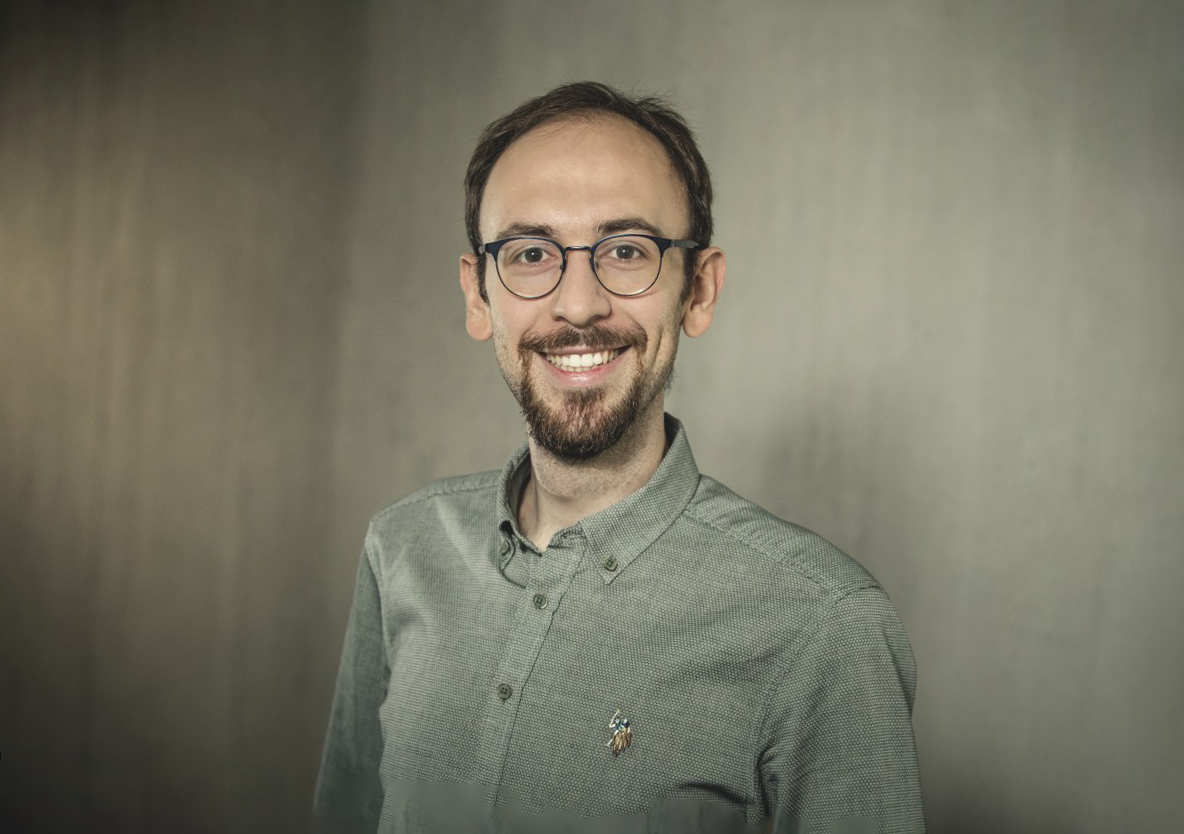
\includegraphics[height=3.1cm]{uploads/resume-portrait.png}};\end{tikzpicture}
\end{minipage}
\cvsection{Res}{earch Interest}
\textbf{Main Areas}\quad Spatial 3D Perception, Embodied AI, State Estimation \& Mapping in the Wild
\cvsection{Edu}{cation}
\education{Ph.D. in Mechanical and Process Engineering (Robotics)}{ETH Zurich}{Robust spatial 3D perception in degenerate environments to enable robot autonomy.\par Supervisors: Prof. Marco Hutter, Dr. Cesar Cadena}{Feb. 2023 – Present}
\education{M.Sc. in Robotics, Systems \& Control}{ETH Zurich}{Thesis: X-ICP: Localizability-Aware LiDAR Registration for Robust Localization in Extreme Environments.}{Sep. 2019 – May 2022}
\education{B.Sc. in Control \& Automation Engineering (Rank: 1st/105)}{Istanbul Technical University}{Thesis: Deep learning frameworks to learn prediction and simulation focused control system models.}{Sep. 2015 – Jun. 2019}
\education{B.Sc. in Mechanical Engineering (Rank: 1st/81)}{Istanbul Technical University}{Thesis: Design and development of FOLLY: A self-foldable and self-deployable quadcopter.}{Sep. 2013 – Jun. 2018}
\cvsection{Pub}{lications}
{\footnotesize * Equal contribution; order within the marked group is a presentation choice.}\par
% Publications start
\cvsubsection{Journal Articles}
\cvpub{\href{https://doi.org/10.1177/02783649261480737}{GrandTour: A legged robotics dataset in the wild for multi-modal perception and state estimation}}{\textbf{Turcan Tuna}\textsuperscript{*}, Jonas Frey\textsuperscript{*}, Lanke Frank Tarimo Fu, Katharine Patterson, Tianao Xu, Maurice Fallon, Cesar Cadena, Marco Hutter}{The International Journal of Robotics Research (IJRR), OnlineFirst, 1 October 2026}{}
\cvpub{\href{https://doi.org/10.1109/LRA.2026.3732906}{TRaIL-Odom: Tightly Coupled Continuous Time Radar-IMU-LiDAR Odometry With Adaptive Doppler Weighting}}{Chiyun Noh, \textbf{Turcan Tuna}, William Talbot, Marco Hutter, Laurent Kneip, Ayoung Kim}{IEEE Robotics and Automation Letters (RA-L), accepted 23 August 2026}{{\fontsize{8}{9.2}\selectfont Accepted 23 August 2026; assigned to the November 2026 issue, 11(11), 12631–12638. Status recorded as of 22 October 2026.\par}}
\cvpub{\href{https://doi.org/10.1109/TRO.2026.3714645}{Holistic Fusion: Task- and Setup-Agnostic Robot Localization and State Estimation With Factor Graphs}}{Julian Nubert, \textbf{Turcan Tuna}, Jonas Frey, Cesar Cadena, Katherine J. Kuchenbecker, Shehryar Khattak, Marco Hutter}{IEEE Transactions on Robotics (T-RO) 42, 3366–3387, 2026}{}
\cvpub{\href{https://doi.org/10.1109/RAP.2026.3702579}{CaRLi-V: Camera–RADAR–LiDAR Point-Wise 3-D Velocity Estimation}}{Landson Guo, Andres M. Diaz Aguilar, William Talbot, \textbf{Turcan Tuna}, Marco Hutter, Cesar Cadena}{IEEE Robotics and Automation Practice 1, 138–143, 2026}{}
\cvpub{\href{https://doi.org/10.1109/TFR.2025.3576053}{Informed, Constrained, Aligned: A Field Analysis on Degeneracy-Aware Point Cloud Registration in the Wild}}{\textbf{Turcan Tuna}, Julian Nubert, Patrick Pfreundschuh, Cesar Cadena, Shehryar Khattak, Marco Hutter}{IEEE Transactions on Field Robotics 2, 485–515, 2025}{}
\cvpub{\href{https://doi.org/10.1109/TRO.2025.3593079}{Continuous-Time State Estimation Methods in Robotics: A Survey}}{William Talbot, Julian Nubert, \textbf{Turcan Tuna}, Cesar Cadena, Frederike Dümbgen, Jesús Tordesillas, Timothy D. Barfoot, Marco Hutter}{IEEE Transactions on Robotics (T-RO) 41, 4975–4999, 2025}{}
\cvpub{\href{https://doi.org/10.1109/TRO.2023.3335691}{X-ICP: Localizability-Aware LiDAR Registration for Robust Localization in Extreme Environments}}{\textbf{Turcan Tuna}, Julian Nubert, Yoshua Nava, Shehryar Khattak, Marco Hutter}{IEEE Transactions on Robotics (T-RO) 40, 452–471, 2024}{}
\cvpub{\href{https://doi.org/10.1126/scirobotics.ade9548}{Scientific exploration of challenging planetary analog environments with a team of legged robots}}{Philip Arm, Gabriel Waibel, Jan Preisig, \textbf{Turcan Tuna}, Ruyi Zhou, Valentin Bickel, Gabriela Ligeza, Takahiro Miki, Florian Kehl, Hendrik Kolvenbach, Marco Hutter}{Science Robotics 8(80), eade9548, 2023}{}
\cvpub{\href{https://doi.org/10.1007/s10489-021-02416-0}{Deep learning frameworks to learn prediction and simulation focused control system models}}{\textbf{Turcan Tuna}, Aykut Beke, Tufan Kumbasar}{Applied Intelligence 52(1), 662–679, 2022}{}
\cvpub{\href{https://doi.org/10.1016/j.ast.2020.105807}{Design and development of FOLLY: A self-foldable and self-deployable quadcopter}}{\textbf{Turcan Tuna}, Salih Ertug Ovur, Etka Gokbel, Tufan Kumbasar}{Aerospace Science and Technology 100, 105807, 2020}{}
\clearpage
\cvsubsection{Conference Proceedings}
\cvpub{\href{https://doi.org/10.15607/RSS.2026.XXII.049}{BIEVR-LIO: Robust LiDAR-Inertial Odometry through Bump-Image-Enhanced Voxel Maps}}{Patrick Pfreundschuh, \textbf{Turcan Tuna}, Cedric Le Gentil, Roland Siegwart, Cesar Cadena, Helen Oleynikova}{Robotics: Science and Systems (RSS), 2026}{}
\cvpub{\href{https://doi.org/10.15607/RSS.2025.XXI.134}{Boxi: Design Decisions in the Context of Algorithmic Performance for Robotics}}{\textbf{Turcan Tuna}\textsuperscript{*}, Jonas Frey\textsuperscript{*}, Lanke Frank Tarimo Fu\textsuperscript{*}, Cedric Weibel, Katharine Patterson, Benjamin Krummenacher, Matthias Müller, Julian Nubert, Maurice Fallon, Cesar Cadena, Marco Hutter}{Robotics: Science and Systems (RSS), 2025}{}
\cvpub{\href{https://doi.org/10.1109/CVPR52734.2025.00624}{ForestLPR: LiDAR Place Recognition in Forests Attentioning Multiple BEV Density Images}}{Yanqing Shen, \textbf{Turcan Tuna}, Marco Hutter, Cesar Cadena, Nanning Zheng}{IEEE/CVF Conference on Computer Vision and Pattern Recognition (CVPR), 2025 — Highlight}{}
\cvpub{\href{https://doi.org/10.1109/ICRA55743.2025.11127534}{Diffusion Based Robust LiDAR Place Recognition}}{Benjamin Krummenacher, \textbf{Turcan Tuna}\textsuperscript{*}, Jonas Frey\textsuperscript{*}, Olga Vysotska, Marco Hutter}{IEEE International Conference on Robotics and Automation (ICRA), 2025}{}
\cvpub{\href{https://doi.org/10.1109/ICRA55743.2025.11128847}{LEVA: A High-Mobility Logistic Vehicle with Legged Suspension}}{Marco Arnold, Lukas Hildebrandt, Kaspar Janssen, Efe Ongan, Pascal Bürge, Ádám Gyula Gábriel, James Kennedy, Rishi Lolla, Quanisha Oppliger, Micha Schaaf, Joseph Church, Michael Fritsche, Victor Klemm, \textbf{Turcan Tuna}, Giorgio Valsecchi, Cedric Weibel, Michael Wüthrich, Marco Hutter}{IEEE International Conference on Robotics and Automation (ICRA), 2025}{}
\cvpub{\href{https://doi.org/10.1109/RoMoCo60539.2024.10604355}{Global Path Planning for Autonomous Vehicles in Orchards and Vineyards}}{Timo Schönegg, \textbf{Turcan Tuna}, Fan Yang, Gabriel Waibel, Matias Mattamala, Marco Hutter}{International Workshop on Robot Motion and Control (RoMoCo), 2024}{}
\cvpub{\href{https://doi.org/10.1109/CEIT.2018.8751883}{FOLLY: A Self Foldable and Self Deployable Autonomous Quadcopter}}{\textbf{Turcan Tuna}, Salih Ertug Ovur, Etka Gokbel, Tufan Kumbasar}{Conference on Control Engineering \& Information Technology (CEIT), 2018 — Best Paper Award}{}
\cvsubsection{Workshop Contributions}
\cvpub{\href{https://arxiv.org/abs/2404.14157}{Autonomous Forest Inventory with Legged Robots: System Design and Field Deployment}}{Matías Mattamala, Nived Chebrolu, Benoit Casseau, Leonard Freißmuth, Jonas Frey, \textbf{Turcan Tuna}, Marco Hutter, Maurice Fallon}{ICRA Workshop on Field Robotics, 2024}{{\fontsize{8}{9.2}\selectfont Accepted to the ICRA 2024 Workshop on Field Robotics.\par}}
\cvsubsection{Preprints}
\cvpub{\href{https://arxiv.org/abs/2603.06691}{One-Shot Badminton Shuttle Detection for Mobile Robots}}{Florentin Dipner, William Talbot, \textbf{Turcan Tuna}, Andrei Cramariuc, Marco Hutter}{arXiv preprint, 2026; submitted to IEEE Robotics and Automation Practice}{{\fontsize{8}{9.2}\selectfont Preprint; journal acceptance not verified as of 22 October 2026.\par}}
\cvpub{\href{https://arxiv.org/abs/2601.07362}{Large-Scale Autonomous Gas Monitoring for Volcanic Environments: A Legged Robot on Mount Etna}}{Julia Richter, \textbf{Turcan Tuna}, Manthan Patel, Takahiro Miki, Devon Higgins, James Fox, Cesar Cadena, Andres Diaz, Marco Hutter}{arXiv preprint, 2026; submitted to IEEE Robotics \& Automation Magazine}{{\fontsize{8}{9.2}\selectfont Preprint; journal acceptance not verified as of 22 October 2026.\par}}
% Publications end
\clearpage
\cvsection{Wor}{k and Research Experience}
\job{Research Exchange}{MA, USA}{MIT — SPARK Lab}{Sep. 2024 – Dec. 2024}
\begin{itemize}\item Research on spatial 3D mapping with Gaussian splatting for a generalizable robotic mapping pipeline.\end{itemize}\vspace{5pt}
\job{Ph.D. Candidate}{Zurich, Switzerland}{ETH Zurich — Robotic Systems Lab}{Feb. 2023 – Present}
\begin{itemize}\item Research on spatial 3D perception in geometrically degenerate environments using multimodal sensors.
\item Develop degeneracy-aware point cloud registration methods and analyze mitigation strategies for SLAM.\end{itemize}\vspace{5pt}
\job{Scientific Researcher}{Zurich, Switzerland}{ETH Zurich — Robotic Systems Lab}{May 2022 – Feb. 2023}
\begin{itemize}\item Independent research on robust localization and mapping for legged robots.
\item Developed X-ICP for localizability-aware LiDAR registration and conducted large-scale evaluation.\end{itemize}\vspace{5pt}
\job{Teaching Assistant — Robot Dynamics}{Zurich, Switzerland}{ETH Zurich, Department of Mechanical and Process Engineering}{Sep. 2022 – Jan. 2023}
\begin{itemize}\item Assisted with lectures and exercises for the Robot Dynamics course (4 ECTS).
\item Prepared and graded assignments and examinations; supported students during lab sessions.\end{itemize}\vspace{5pt}
\job{Perception Engineering Intern}{Zurich, Switzerland}{ANYbotics AG}{Mar. 2021 – Oct. 2021}
\begin{itemize}\item Implemented global initialization and robust localization/mapping for ANYmal quadrupedal robots.
\item Integrated LiDAR, camera and inertial sensors for sensor-fusion odometry.
\item Conducted field trials in multifloor facilities and on rough terrain.\end{itemize}\vspace{5pt}
\job{Student Mechanical Designer}{Zurich, Switzerland}{Autonomous Systems Lab, ETH Zurich}{Sep. 2019 – Mar. 2021}
\begin{itemize}\item Redesigned Super Mega Bot for the DARPA Subterranean Challenge, focusing on robustness and maintainability.
\item Performed mechanical design, optimization and finite element analysis; oversaw manufacturing and assembly.\end{itemize}\vspace{5pt}
\job{Research Assistant}{Istanbul, Turkey}{Istanbul Technical University}{Sep. 2018 – Jun. 2019}
\begin{itemize}\item Worked on deep learning for nonlinear system identification and time-series prediction.
\item Co-authored the journal article on prediction- and simulation-focused models for control systems.\end{itemize}\vspace{5pt}
\job{Research Intern}{London, United Kingdom}{Imperial College London}{Jun. 2018 – Sep. 2018}
\begin{itemize}\item Developed algorithms to infer mental states using visual and biosignal data for human–robot interaction.
\item Combined EEG, EMG and video data in machine-learning pipelines to estimate human stress levels.\end{itemize}
\cvsection{Tea}{ching}
\award{2022–}{ETH Zurich — Robotics Summer School lecturer and teaching assistant.}
\award{2023–}{ETH Zurich — Master's thesis and semester project supervision.}
\award{2022–23}{ETH Zurich — Robot Dynamics teaching assistant.}
\cvsection{Awa}{rds}
\award{2025}{CVPR Highlight — ForestLPR: LiDAR Place Recognition in Forests Attentioning Multiple BEV Density Images.}
\award{2024}{RoMoCo Young Author Best Paper Award — Global Path Planning for Autonomous Vehicles in Orchards and Vineyards; Timo Schönegg received the award for the co-authored paper.}
\award{2021}{ISIF Silver Medal — with Etka Gökbel and Salih Ertuğ Övür, for a patent registered in Turkey.}
\award{2018}{CEIT Best Paper Award — FOLLY: A Self Foldable and Self Deployable Autonomous Quadcopter.}
\award{2019}{Top Graduate — Control \& Automation Engineering, Istanbul Technical University (1st/105).}
\award{2018}{Top Graduate — Mechanical Engineering, Istanbul Technical University (1st/81).}
\cvsection{Ser}{vice and Invited Talks}
\award{2026}{IROS workshop organizer — Data in Field Robotics: From State Estimation to Navigation, 1 October.}
\award{2025}{INTERGEO talk — GrandTour and Boxi, 9 October.}
\award{2025}{Scientific keynote, FZI RimA Summer School — Towards Walking Robots in Domestic Environments, 13 August.}
\end{document}
